%%%%%%%%%%%%%%%%%%%%%%%%%%%%%%%%%%%%%%%%%
% Memo
% LaTeX Template
% Version 1.0 (30/12/13)
%
% This template has been downloaded from:
% http://www.LaTeXTemplates.com
%
% Original author:
% Rob Oakes (http://www.oak-tree.us) with modifications by:
% Vel (vel@latextemplates.com)
%
% License:
% CC BY-NC-SA 3.0 (http://creativecommons.org/licenses/by-nc-sa/3.0/)
%
%%%%%%%%%%%%%%%%%%%%%%%%%%%%%%%%%%%%%%%%%

\documentclass[letterpaper,11pt]{texMemo} % Set the paper size (letterpaper, a4paper, etc) and font size (10pt, 11pt or 12pt)

\usepackage{parskip} % Adds spacing between paragraphs
\usepackage[colorlinks]{hyperref}
\usepackage{graphicx}
\usepackage{float}
\usepackage{listings}
\hypersetup{citecolor=DeepPink4}
\hypersetup{linkcolor=red}
\hypersetup{urlcolor=blue}
\usepackage{cleveref}
\setlength{\parindent}{15pt} % Indent paragraphs

%----------------------------------------------------------------------------------------
%	MEMO INFORMATION
%----------------------------------------------------------------------------------------

\memoto{Dr.Randy Hoover} % Recipient(s)

\memofrom{Benjamin Lebrun, Benjamin Garcia} % Sender(s)

\memosubject{Lab Assignment 2: AVR Assembly and UART Communication} % Memo subject

\memodate{\today} % Date, set to \today for automatically printing todays date

%\logo{\includegraphics[width=0.1\textwidth]{logo.png}} % Institution logo at the top right of the memo, comment out this line for no logo

%----------------------------------------------------------------------------------------

\begin{document}

\maketitle % Print the memo header information

%----------------------------------------------------------------------------------------
%	MEMO CONTENT
%----------------------------------------------------------------------------------------

\section*{Introduction}
%This section \textit{briefly} communicates what you have been asked to accomplish in the lab, how you approached it, and what results you saw. This is \textbf{not} an area for manifestos.
This lab required us to output the value in a counter to three LEDs as well as to the UART serial port. Additionally, we were required to accept input from the serial port and use this input to set the value of the counter. A component of the output requirement was that it print/flash the LEDs every two seconds using a wait function that we created.

Our implementation holds the counter in a register and converts to and from an ASCII representation for presenting information over the serial port. Pins 0, 1, and 2 on PORTB were used for lighting up the LEDs. To handle receiving information over the serial port, we enabled the 'UART RX Complete interrupt' so that whenever a key is pressed, it will set the value of the counter for the next time the LEDs are flashed. Our wait uses a triply nested loop to consume 16,000,000 cycles (1 second when running at 16MHz).

The finished implementation blinks on a two second cycle (two seconds on, two seconds off) and key-presses are registered for the next cycle. When first turned on, the counter is initially set to 0, and the LEDs are off.


\section*{Equipment}
This lab required the following equipment:
\begin{itemize}
\item 3 resistors (220$\Omega$)
\item 3 LEDs
\item 4 wires (male-male)
\item 1 USB-A to USB-B cable
\item 1 breadboard
\item 1 Arduino UNO (ATMega328P)
\item Atmel Studio 7
\item Putty
\end{itemize}

\subsection*{configuration}
The Arduino was connected to the computer with the USB-A to USB-B cable. On the breadboard, each LED was placed in a circuit with a single resistor connected to ground. One of the Arduino's ground pins was connected to the breadboard's ground, and the LEDs were connected to PORTB pins 0, 1, and 2 (pins numbered 8, 9, 10 on the Arduino).

\begin{figure}[!ht]
\begin{center}
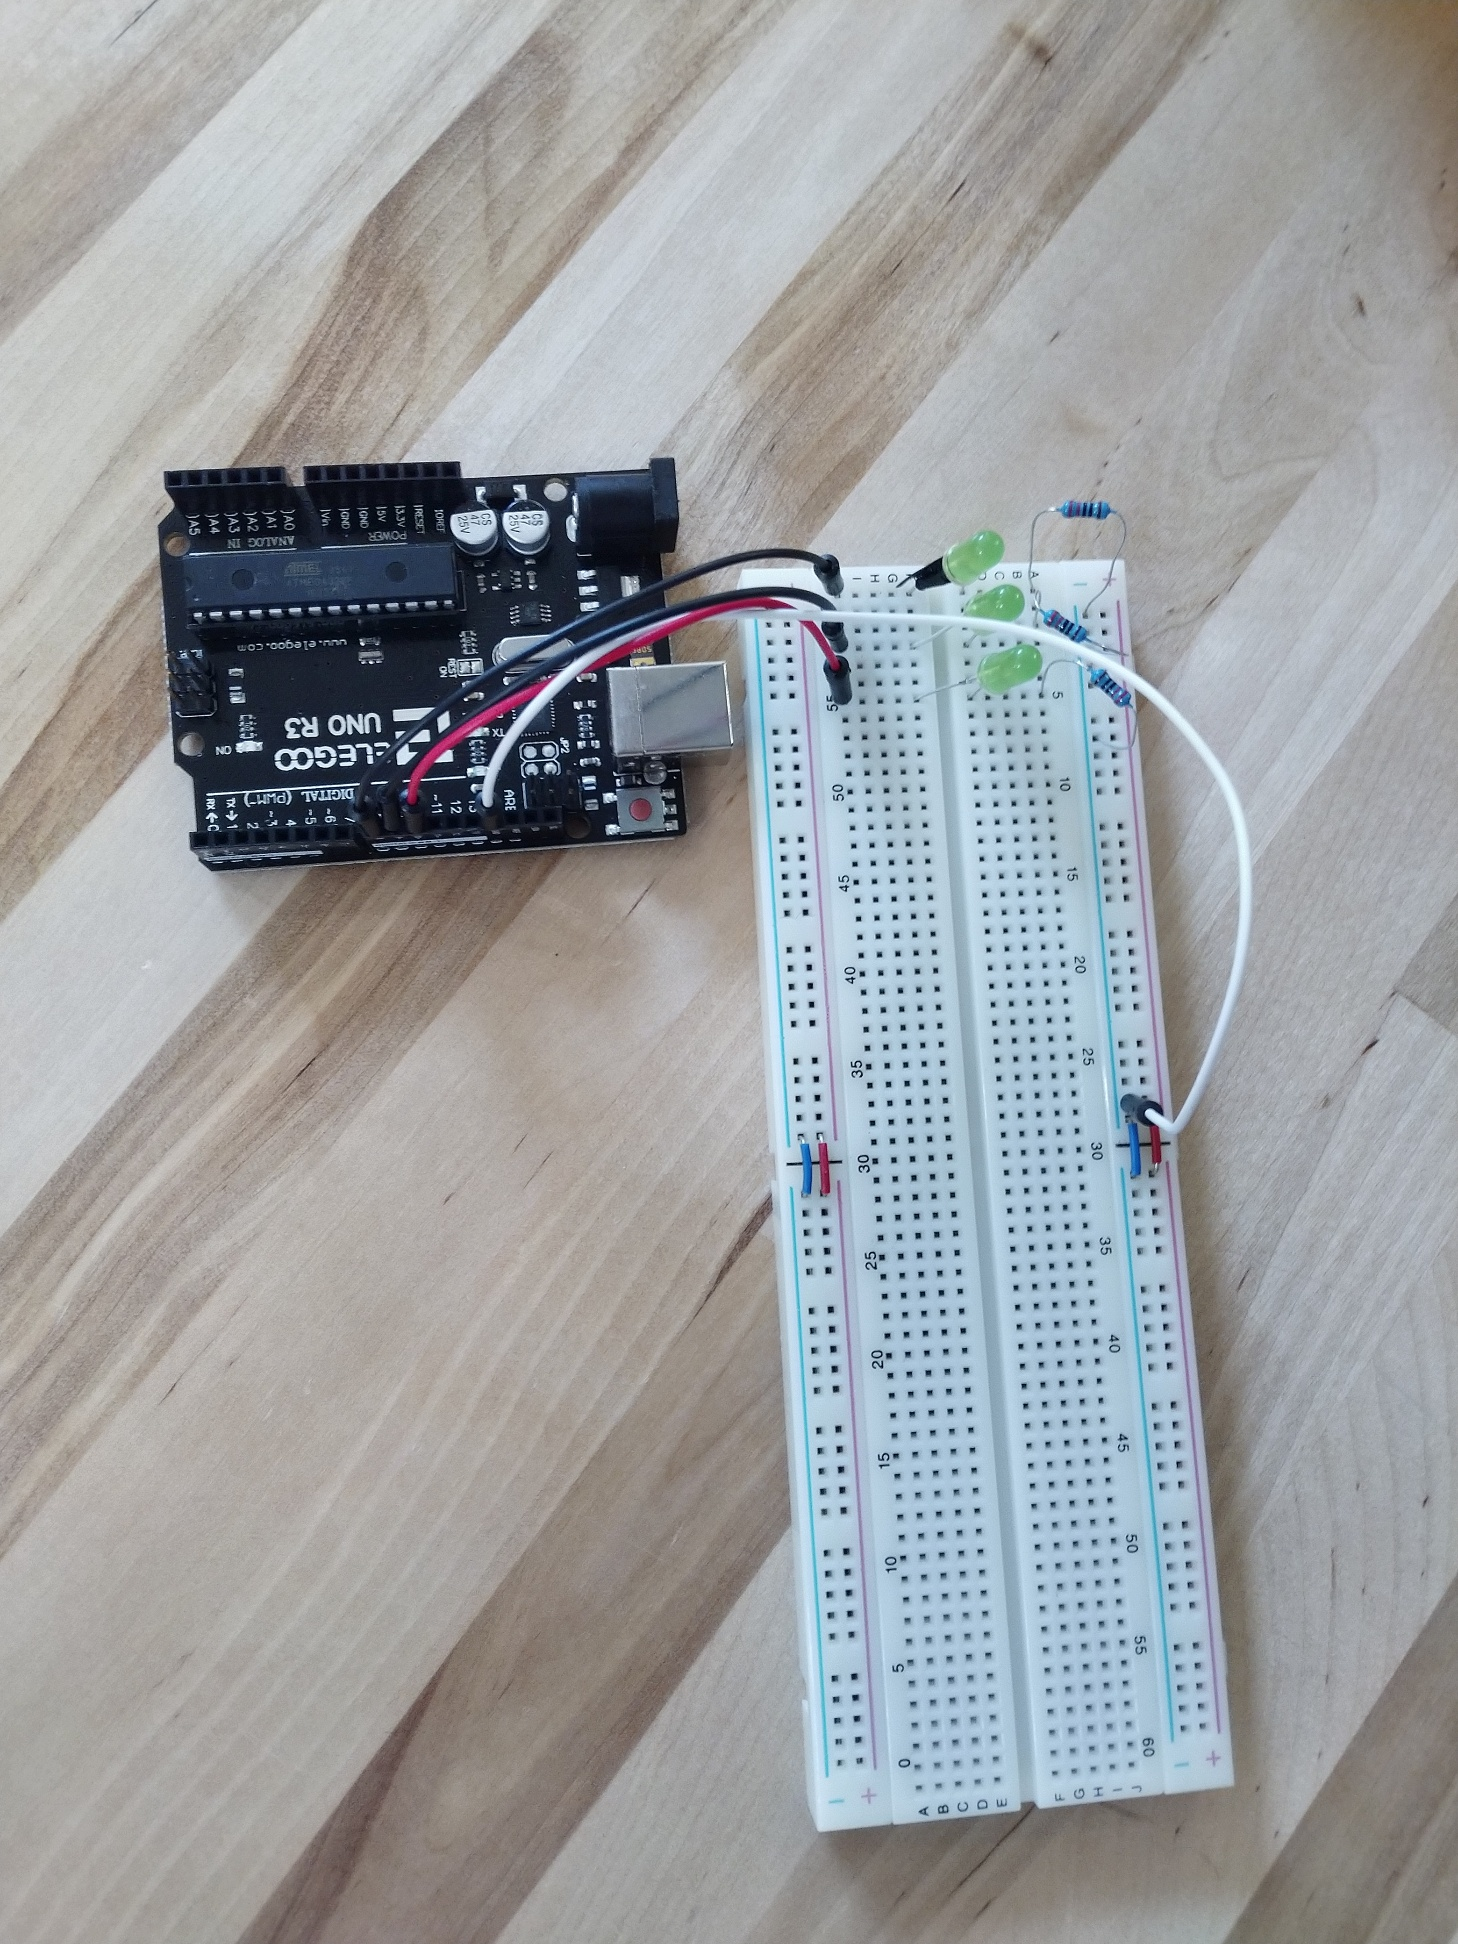
\includegraphics[scale=0.25]{./configuration.jpg}
\caption{Picture of the wiring setup}
\end{center}
\end{figure}

\newpage
\section*{Implementation}
\subsection*{One Second Wait}
The wait implementation uses three registers as loop variables to create a busy loop that occupies 15,999,984 cycles with variable pushing and popping and the function's return occupying a further 16 cycles to give 16,000,000 cycles.

\subsection*{ATOI}
Handles converting numbers in ASCII representation to their depicted value (i.e. '7' is converted from 0x37 to 0x07).

It subtracts '0' (0x30) from the incoming ASCII character value to produce the numeric value. Once this is done, the value is stored in the counter for use on the next light cycle.

\subsection*{ITOA}
Does the exact opposite of ATOI, it converts a numeric value to an ASCII character (i.e. 0x07 converts to 0x37 '7').

This is accomplished by subtracting the quantity (0 - '0') from the number (equivalent to adding 0x30). This value is sent over the serial line to the computer, where Putty can display it.

\subsection*{UART\_RX (Interrupt)}
To handle the RX complete interrupt, we first altered the Init code provided to set UCSR0B to 0x98 to enable bits 7 (RX Complete Interrupt), 4 (RX Enable), and 3(TX Enable). Once the global interrupt bit was set, our function 'UART\_RX' would be called whenever the UART buffer was filled. This function calls ATOI to set the counter and then returns control to the last instruction executed.

\subsection*{UART\_INIT}
UART\_INIT is boilerplate code that was provided with the lab. The only change we have made is to enable the 'RX Complete Interrupt' as mentioned above.

This function configures the UART control and status registers to allow writing and reading using the '8n1' protocol on the UART port. Additionally, communication is configured to use a baudrate of 9600.

\subsection*{UART\_TX}
Unlike the RX function, UART\_TX is not an interrupt, and is called every time the 'flash\_leds' function is called. This function waits until the buffer is empty to write, then calls itoa to convert the counter to an ASCII character and outputs it to the serial port.

\subsection*{Program Loop and Startup}
Our startup routine first assigned 0xff to DDRB to enable output. Then we initialize our counter to 0, and setup the stack to begin at RAMEND. Finally, we call the UART\_INIT function to configure the UART for the Program Loop.

The Program Loop starts by waiting for two seconds, then it will flash the LEDs, outputting the value of our counter to the LEDs and the serial port. Then, two seconds later, it turns off the LEDs. After the LEDs have been turned off, we jump back to the start of the Program Loop.

\section*{Discussion}
AVR assembly is an uncomplicated approach to the larger family of assembly architectures. We have access to a decently sized array of registers but also can access special hardware and software features usually by a call to a memory address on the board.

Our first smaller issue was remembering how to convert between ASCII codes and a normal integer value. After rewriting the transmit method from the lab handout, we mistakenly sent ASCII codes being subtracted from zero into the UART, which displayed an invalid character to the screen. This was remedied by simply remembering the correct conversion between integers and ASCII codes.

To implement the receive function, we used interrupts instead of waits or delays to properly receive data. The transmit function, because of the nature of our application, could be called in code with every flash of the LEDs at the prescribed interval from our lab requirements and specs and therefore did not require the direct use of an interrupt to constantly check the state of the buffer or carefully navigate writing to the assigned register buffer.  However, we found out that simply setting the global interrupt flag and creating our interrupt vectors in code wasn’t enough to activate the interrupt. As noted in implementation we also had to set a specified interrupt flag to activate the correct interrupt.

\newpage
\section*{Responses}
Respond intelligently and at necessary length to any questions posed in the lab assignment.
\begin{enumerate}

\section{It is extremely unlikely that your one-second delay is exactly one second. How many clock
cycles are actually consumed inside your one-second delay? What is your relative error?}

\item Our wait uses exactly 16 Million cycles plus 3 for the initial call. Our function does account for the two cycles used if our break if equal command does attempt to set the comparison register. For 16 million cycles on our board with three for the call, our delay lasts for 16,000,003 cycles comes within 0.18 nanoseconds of one second, or approximately 0.00001875\% error.

\section{The USB serial communication protocol and the UART communication we’ve implemented
on the ATMega328P are very different, yet we are able to plug a cable between the two and
communicate! How is this possible on the Arduino Uno R3?}

\item The Arduino Uno R3 uses a dedicated memory address to write to a built-in USB to serial adaptor. This adaptor has a specialized chip which attempts to carry UART communication through USB protocol, and generally has its own built in EEPROM, voltage regulators, receivers and transmitters and internal timing oscillator and a host of other features to allow communication conversion between USB and UART.

\section{Explain each step of the UART RX call provided in this document.}

\item UART RX first pushes the contents of register 17 onto the program stack for storage, then loads the status of the UART buffer from the UCSR0A register. We use this register to read the status of the UART, such as if the buffer is full or if communication has ended. In our case we are waiting for communication to end and compare the RCX0 register to do this. We use a comparison to check if this bit is set; if it is, we then load the contents of the UDR0 data register into register 16. Then we pop the data from the program stack back onto register 17 where we previously carried our UART status register and carry on.

\end{enumerate}

\section*{Appendices}
The following files are included as appendices:
\begin{itemize}
\item main.asm
\item wait2.asm (the version of the wait function used in the program)
\end{itemize}
\newpage

\section*{Appendix A: main.asm}
\begin{tiny}
\lstinputlisting{../main.asm}
\end{tiny}
\newpage
\section*{Appendix B: wait2.asm}
\begin{tiny}
\lstinputlisting{../wait2.asm}
\end{tiny}
\end{document}
\grid
